%----------------------------------------------------------------------------------------
%	Monte Carlo method for estimating Pi using OpenMP
%----------------------------------------------------------------------------------------

\section{Monte Carlo method for approximating the value of $\pi$ in OpenMP}

\subsection{Compile and run the template code with a single thread, and thus verify that the serial
version is correct.}

\begin{figure}[ht]
    \centering
    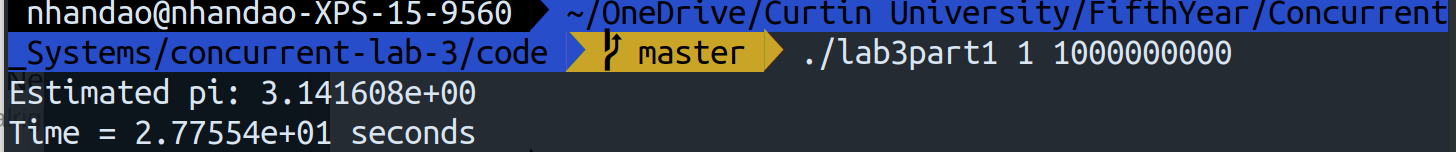
\includegraphics[width=\textwidth]{graphics/P1_a_terminal_output.png}
    \caption{Terminal output of execution of template code with a single thread}
    \label{fig:P1_a_term_out}
\end{figure}

\subsection{Parallelize the code for multi-threaded execution by ONLY adding OpenMP directives}

\vspace{0.5cm}
\lstinputlisting[
	style=CStyle,
	firstline=34, % First line of code
	lastline=48, % Lastl ine of code
	caption=Parallizing the code for multi-threaded execution (line 34-48 in lab3part1.c), % Caption above the listing
	label=lst:lab3part1a, % Label for referencing this listing
	frame=single, % Frame around the code listing
	showstringspaces=false, % Don't put marks in string spaces
	numbers=left, % Line numbers on left
	numberstyle=\normalsize % Line numbers styling
    ]{../code/lab3part1.c}
    
\subsubsection{At what point in the code new threads are forked and joined?}
The code is serial up until \emph{pragma}. At pragma, multiple threads are forked,
line 1 in \cref{lst:lab3part1a}. After the structured block (line 2 - 15), the slaves are joined with 
the master thread and execution resumes on the master thread.

\subsubsection{Which part of the code is executed by which threads?}
The total number of threads are comprised of one main thread, and the remainder are slave threads.
The main thread will run all code outside of the parallel enivornment. Master and slaves thread will 
run the section of code assigned by the OpenMP directives - line 2 - 15.

\subsubsection{Where barrires if any in terms of thread synchronization would be encountered,
and hence how the code achives parallelization}
write something